\section{Context Growth, Reconstruction Cost, and State Economics}
\label{sec:cost}

RaS has an economic motivation, but the current controlled evidence does not establish monetary savings. The hostile audit therefore separates a theoretical stress model, observable resource accounting, and unobservable provider-internal economics.

\subsection{Full-history replay is a stress model, not the persistent-agent baseline}

Let $B$ be fixed base context, $g$ the average number of new historical tokens added per step, and $n$ sequential reasoning steps. Under \emph{naive full-history replay}, step $i$ receives:
\begin{equation}
T_i=B+g(i-1),
\end{equation}
so cumulative supplied input is:
\begin{align}
T_{\mathrm{full}}(n)
&=\sum_{i=1}^{n}[B+g(i-1)] \\
&=nB+\frac{gn(n-1)}{2}
\in\Theta(n^2)
\end{align}
for fixed $g>0$.

This is correct algebra but a weak empirical baseline. Modern agents may use prefix caching, context windows, compaction, summaries, retrieval, selective history, server-side state, or other mechanisms. Let $h_i^*$ be the effective historical input supplied to a persistent reasoner after such management. Then:
\begin{equation}
T_{\mathrm{persistent}}(n)=\sum_{i=1}^{n}(B+h_i^*).
\label{eq:persistent-general}
\end{equation}
If $h_i^*$ is bounded, persistent cumulative supplied input is also linear in $n$. Consequently, \textbf{there is no general asymptotic RaS advantage over a well-managed persistent agent}. The quadratic curve is retained only as a theoretical full-replay stress case.

For RaS, let $K_i$ be reconstructed repository/task input:
\begin{equation}
T_{\mathrm{RaS}}(n)=\sum_{i=1}^{n}K_i.
\end{equation}
The original bounded assumption $K_i\le K$ is also only a stress model. A more realistic reconstruction size is:
\begin{equation}
K_i=f(|R_i|,L_i,D_i,Q_i^{\mathrm{doc}},Q_i^{\mathrm{test}},Q_i^{\mathrm{arch}},Q_i^{\mathrm{retrieval}}),
\label{eq:realistic-k}
\end{equation}
where repository size, task locality, dependency width, and documentation/test/architecture/retrieval quality can all affect rediscovery.

Figure~\ref{fig:context-growth} therefore illustrates two conditional mathematical shapes, not an empirical comparison of deployed agents.

\begin{figure}[htbp]
\centering
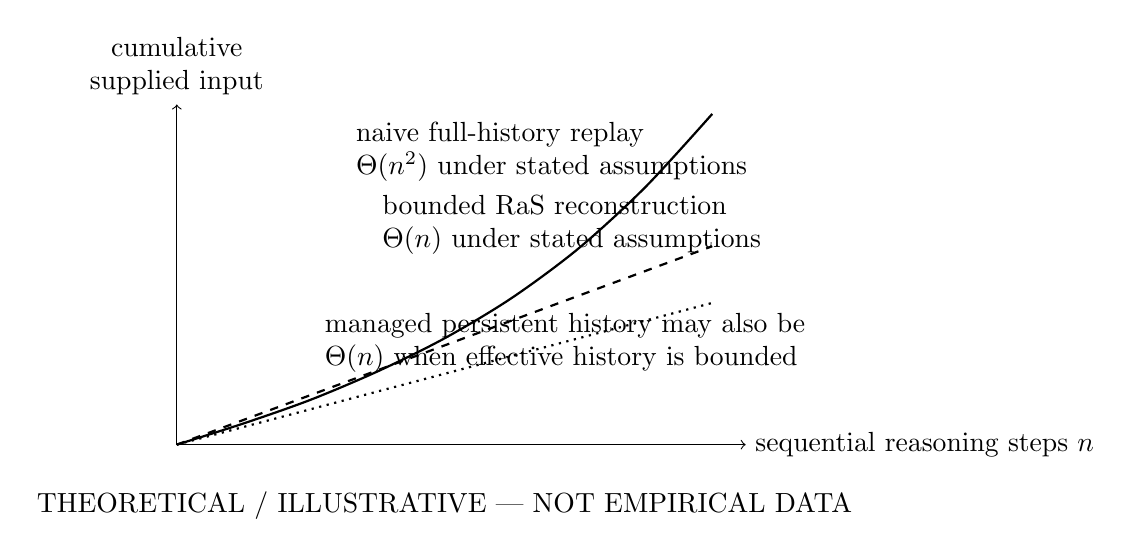
\begin{tikzpicture}[x=0.85cm,y=0.6cm]
\draw[->] (0,0) -- (8.5,0) node[right]{sequential reasoning steps $n$};
\draw[->] (0,0) -- (0,7.2) node[above,align=center]{cumulative\\supplied input};
\draw[thick] plot[smooth] coordinates {(0,0) (1,0.45) (2,0.95) (3,1.55) (4,2.25) (5,3.1) (6,4.15) (7,5.45) (8,7)};
\draw[thick,dashed] (0,0) -- (8,4.2);
\draw[thick,dotted] (0,0) -- (8,3.0);
\node[align=left] at (5.6,6.2) {naive full-history replay\\$\Theta(n^2)$ under stated assumptions};
\node[align=left] at (5.9,4.65) {bounded RaS reconstruction\\$\Theta(n)$ under stated assumptions};
\node[align=left] at (5.8,2.15) {managed persistent history may also be\\$\Theta(n)$ when effective history is bounded};
\node[below,align=center] at (4,-0.8) {THEORETICAL / ILLUSTRATIVE --- NOT EMPIRICAL DATA};
\end{tikzpicture}

\caption{THEORETICAL / ILLUSTRATIVE --- NOT EMPIRICAL DATA. Quadratic growth is the naive full-history replay stress case; bounded reconstruction is a conditional RaS stress case. Persistent agents with bounded effective history can also have linear cumulative supplied input.}
\label{fig:context-growth}
\end{figure}

\subsection{Rediscovery is allowed to defeat RaS}

Handoff Debt provides direct evidence that repository-only successor agents can pay substantial rediscovery cost after interrupted tasks \citep{kc2026handoff}. RaS does not explain this away: if the same effect remains large after \emph{accepted} transition boundaries, it weakens the practical thesis.

Future experiments should capture:
\begin{itemize}
    \item reconstruction-attributed input tokens;
    \item repository bytes and number of files inspected;
    \item repository, symbol, dependency, and history searches;
    \item model and tool calls;
    \item reconstruction elapsed time and total task elapsed time;
    \item observable cache hits/misses or cached/uncached tokens;
    \item retries and escalations attributable to missing or incorrect reconstruction.
\end{itemize}

The proposed Reconstruction Token Fraction remains descriptive:
\begin{equation}
\mathrm{RTF}=
\frac{T_{\mathrm{reconstruction,input}}}
{T_{\mathrm{RaS,total~input}}}.
\label{eq:rtf}
\end{equation}
RTF alone cannot establish efficiency: a low fraction can coexist with high total cost, and a high fraction can be acceptable if total outcome-normalised resource use is low. Report the numerator and denominator as well as the ratio.

\subsection{Do not double-count conceptual cost components}

The original additive equations risked treating reasoning, context, and agent-state cost as mutually exclusive even though provider billing and inference work can overlap those concepts. The audit replaces them with a measured resource vector:
\begin{equation}
\mathbf{Z}_c=
(T_{\mathrm{in}},T_{\mathrm{out}},N_{\mathrm{model}},N_{\mathrm{tool}},
B_{\mathrm{repo-read}},N_{\mathrm{files}},t_{\mathrm{recon}},t_{\mathrm{total}},
N_{\mathrm{retry}},C_{\mathrm{billed}})
\label{eq:resource-vector}
\end{equation}
for condition $c$, with elements reported only where observable and with $C_{\mathrm{billed}}$ included only when exposed by the provider or metered service.

\begin{table}[htbp]
\centering
\small
\caption{Audit classification of economic/resource quantities. “Observable” means available to the experiment, not necessarily a direct measure of provider-internal cost.}
\label{tab:cost-observability}
\begin{tabularx}{\textwidth}{@{}lX X@{}}
\toprule
Class & Examples & Permitted use \\
\midrule
OBSERVABLE & Input/output tokens exposed by API, model/tool calls, repository bytes/files read, searches, elapsed time, retries, provider-billed charge when exposed & Report directly; compare outcome-normalised values across conditions \\
PARTIALLY OBSERVABLE & Cached-token counters, prompt-cache hits, session persistence indicators, opaque provider usage categories & Report with interface/version and limitations; do not infer hidden implementation \\
UNOBSERVABLE & Exact GPU allocation, KV-cache residency cost, internal storage/scheduling amortisation, provider margin & Do not label as measured saving; discuss only as theoretical implication \\
\bottomrule
\end{tabularx}
\end{table}


A monetary comparison may sum \emph{mutually exclusive metered charges} actually observed by the experiment. It must not add speculative “reasoning cost”, “KV-cache cost”, “GPU cost”, and subscription price as if those were independent measured quantities.

Three categories remain:
\begin{itemize}
    \item \textbf{OBSERVABLE}: experiment-side tokens/calls/reads/times and provider-billed usage when exposed;
    \item \textbf{PARTIALLY OBSERVABLE}: cache behaviour, retained session state, or provider-reported categories whose implementation is not transparent;
    \item \textbf{UNOBSERVABLE}: internal GPU scheduling, exact KV-cache residency cost, storage amortisation, hidden cache implementation, and provider margin.
\end{itemize}

LLM-serving research shows that KV-cache management and prefill/decode scheduling affect throughput \citep{kwon2023vllm,zhong2024distserve,qin2024mooncake}. It does \emph{not} justify inferring that closing a conversation releases a dedicated GPU allocation or that RaS yields a particular infrastructure saving. Infrastructure effects remain conditional implications requiring separate serving experiments.
